%% content.tex
%%

%% ==============
\chapter{Dashboard}
\label{ch:Dashboard}
%% ==============

The main goal of our seminar work was to implement a gesture recognition program with which we can reliably control applications like dashboards on the computer.
Therefore, we created a test dashboard with which we examined the usability of our program.
It consists of several diagrams, which can be modified by steering elements like a dropdown menu and radio buttons.
\todo{The main characteristic of the dashboard is that it can be controlled only with the keyboard buttons “tab”, “up”, “down”, “spacebar”, and “enter”.
This makes the steering with our gesture recognition program easier since we can use the python package “pyautogui” to translate recognized gestures into keyboard commands.}

Of course, this is just a simplified example of a dashboard with only a few features compared to what can be found in actual corporate dashboards, which allow more sophisticated commands.
Nevertheless, our dashboard can be easily extended with further features by implementing more steering elements like slide bars or check buttons and by adding more recognizable gestures with which these elements can be controlled.  

\begin{figure}[htp]
\begin{center}
  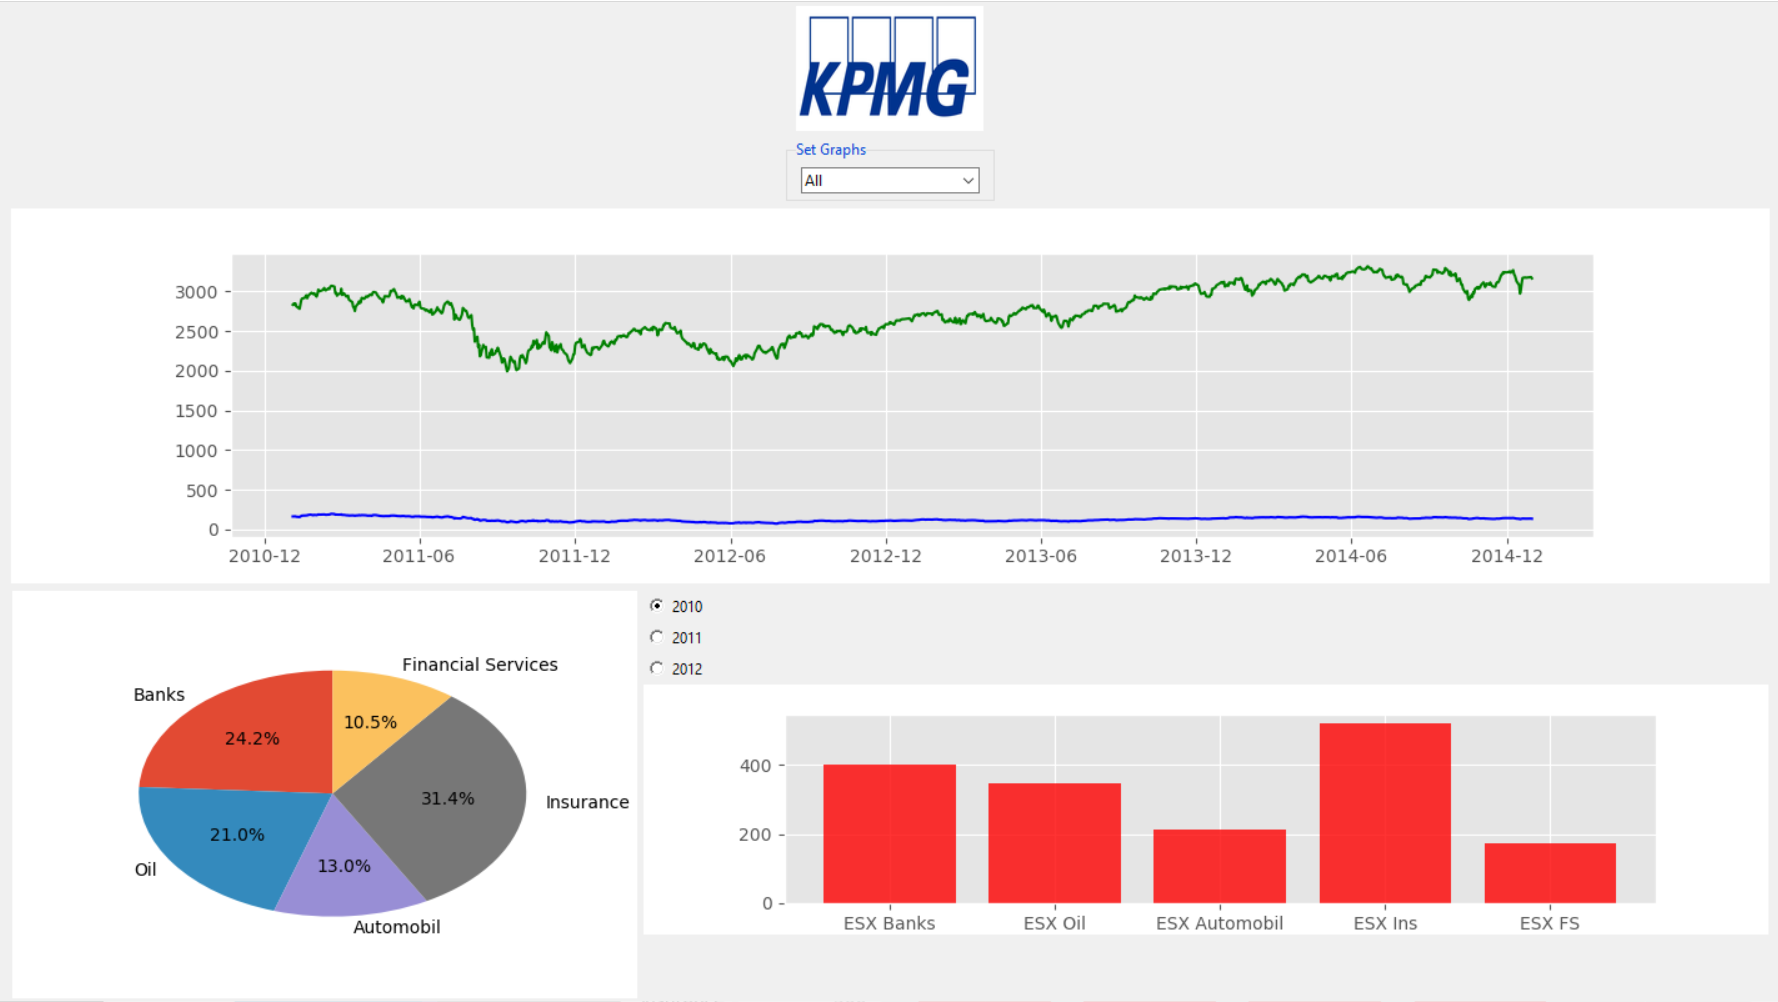
\includegraphics[width = \textwidth]{dashboard.png}
\caption{Our demo application front end}
\end{center}
\end{figure} 


%% ==============
\chapter{System Design}
\label{ch:SystemDesign}
%% ==============

\dots


%% ===========================
\chapter{Data Collection \& Manipulation}
\label{ch:DataCollection}
%% ===========================

Working  with  machine  learning  algorithms  requires  certain  actions  in  order  to choose, prepare and classify data streams.
Choosing the right data is the key decision in order to be able to train the  algorithm properly.
In addition to this  step, preparing data and transforming it into “features” is equally important. 

%% ===========================
\section{Data Collection}
\label{ch:DataCollection:sec:DataCollection}
%% ===========================

To  define  which  data  will  be  collected  we  had  to  think  about  which  kind  of gestures  we  will  want  to  recognize.
Attaching  the  sensors  to  the  back  of  our  hand enables us to observe acceleration data  for x,  y, and z axis  as well  as tilt  angles  alpha, beta and gamma.
We thought about attaching a magnet to our thumb so that we can use the hall-sensor as well,  but we decided to leave this  for  further research.
The collected acceleration and tilt angle data can later be used to distinguish gestures from each other.
To avoid recording and scanning data observed during normal gesticulation we require the acceleration vector length of each gesture to exceed a certain threshold.
In our code we set this treshold to 1.2 G.

%% ===========================
\section{Feature Design}
\label{ch:DataCollection:sec:FeatureDesign}
%% ===========================

Before we can train our algorithm, we  have to transform the recorded data into a set  of  features.
Choosing  and  designing  those  features  affects  the  performance  of  the gesture recognition algorithm heavily.

%% ===========================
\subsection{Preprocessing}
\label{ch:DataCollection:sec:FeatureDesign:sub:Preprocessing}
%% ===========================

Standardization,     scaling,     normalization     and     binarization     are     common preprocessing techniques.
Though, as the acceleration vector and tilt angel sizes are key characteristics  to  distinguish  gestures  scaling,  normalization  and  binarization  are  not applicable for our use case. 

%% ===========================
\subsection{Features}
\label{ch:DataCollection:sec:FeatureDesign:sub:Features}
%% ===========================

\todo{Add images of feature selection}
We  first  thought  about  using  the  variance  as  a  feature,  but  early  tests  already revealed  that  the  acceleration  data  often  has  a  variance  near  zero  and  thus  gives  us almost no information about the executed gesture.

Instead,  maximum  and  minimum  acceleration  per  axis  differ  widely  across gestures  and  are  worth  adding  to  our  feature  set.
To give our classifier a idea of which minimum/maximum was the first, we put them in the right order, so if we have a maximum first, this will be the first feature and the miniumum will become the second feature.
For  instance,  swiping  left  first  shows  a negative  minimum  acceleration, e.g. -1.7G, and then a positive  maximum acceleration, e.g. 1.2G, on the x axis.
We now pick those values out of our buffer and figure out which one was earlier, so we can put them in our feature vector in the right order.
In  this example, we end up with the tuple (-1.7, 1.2).

To include the tilt angles into our feature set, we had to come up with a different approach.
Not only was their variance near zero, but also their minimum and maximum values  are  often  equally  great  across  different  gestures. 
Summing  up  all  angles  led  to non-satisfying  results,  so  we  collect  now  two  features  per  angle:
One  sums  up  the absolute  values  of  negative  angle  differences  and  the  other  one  sums  up  the  absolute values  of  the  positive  angle  differences.
Comparing  both  approaches  the  latter  one increased our average precision  score by ~6\%.
\todo{Include stats “First Approach” vs “Final Solution” here}

%% ===========================
\section{Data Classification}
\label{ch:DataCollection:sec:DataClassification}
%% ===========================

\dots

